\documentclass[../thesis.tex]{subfiles}
\begin{document}\label{sec:3}

Данная глава посвящена сравнению описанных выше стратегий. В ней описывается подготовка необходимых тестовых данных, приведены результаты экспериментов с применением стратегий на этих данных, и сделаны соответствующие выводы.

\subsection{Подготовка тестовых данных}\label{dataset}

Тестовые данные для этой работы состоят из двух частей. Первая, синтетическая, была написана специально для этой работы и представляет собой несколько наборов функций, в каждом из которой размер и сложность функций равномерно увеличивается по заданному шаблону. Вторая часть взята из реальной практики верификации смарт-контрактов.

Для того чтобы синтетические данные подходили для численных экспериментов, необходимо было создать логически несложный код, который может повторяться с незначительными изменениями неограниченное число раз. Вместе с этим необходимо было протестировать такие фундаментальные элементы языков программирования, как условные переходы и рекурсия. В то же время циклы не были включены в этот код, поскольку верификация кода с циклами является отдельной областью исследований, ставящих множество уникальных вопросов \cite{loops_are_hard}, и выходит за рамки этой работы.

Для построения синтетических тестовых данных был выбран классический алгоритм подсчёта полиномиального хеша строки. Этот алгоритм был реализован на языке Ursus в различных вариациях. При этом для этих алгоритмов верифицируется соответствие реализации референсной реализации на языке Coq. Синтетический набор состоит из следующих наборов функций:

\begin{itemize}
    \item \textbf{Simple}. $i$-я функция вычисляет хеш первых $i$ символов строки, при этом код является линейным (не использует циклы или рекурсию), то есть размер кода линейно зависит от порядкового номера функции.
    \item \textbf{If}. Расширение набора \textbf{Simple}, в котором симулируется работа с нуль-\\ терминированными строками. В случае, если программа дошла до нулевого символа, вычисление должно завершиться. Этот набор позволяет протестировать условный оператор и досрочный выход из функции.
    \item \textbf{Recursion}. Рекурсивная версия набора \textbf{Simple}. В ней функция с номером $i+1$ сначала вызывает функцию $i$, а затем дополняет вычисление $(i+1)$-м символом.
    \item \textbf{IfAndRecursion}. Рекурсивная версия набора \textbf{If}.
\end{itemize}

Для реальной части тестовых данных был выбран кошелек с мультиподписью из экосистемы TON \cite{multisig}. Кошельки с мультиподписью используются в блокчейн-сетях повсеместно \cite{wallets_survey} и являются критическим элементом для безопасности многих систем, поэтому верификация таких кошельков имеет практическую значимость. Материалы для верификации этого смарт-контракта были взяты из практики компании Pruvendo, в том числе трансляция кода с исходного языка Solidity на Ursus и формальная спецификация этой системы. Эксперименты заключались в применении разных стратегий для доказательства имеющейся формальной спецификации.

Все эксперименты поставлены на процессоре Intel Xeon E5-2687W v4 @ 3.00GHz с 512 Гб оперативной памяти и 48 ядрами, использовалась версия Coq 8.16.1.

\subsection{Эксперименты на линейном и рекурсивном коде}\label{main_results}

Начнём сравнение стратегий с выявления наименее производительных стратегий, которые определённо не подходят к применению на практике, поскольку работают относительно долго даже на тестах небольшое размеров. Такими стратегиями являются все стратегии, основанные на базовых стратегиях \texttt{bottomup} и \texttt{bottomup-reductions}. На рисунке \ref{plot_bottomup} приведены результаты этих стратегий на наборе тестов Simple. Тогда как стратегия \texttt{native-lazy}, приведённая на этих графиках для сравнения, вычисляет систему уравнений размера 10 за минуту, вычисления для \texttt{bottomup} во всех вариациях и со всеми оптимизациями не укладываются в пять минут на тесте размера 4, а для \texttt{bottomup-reductions}~--- уже на тесте размера 2. На этих и дальнейших графиках вычисления ограничены пятью минутами, то есть измерения в 300 секунд означают превышение этого лимита. 

\graphicspath{ {../images/} }

\begin{figure}[h]
    \begin{subfigure}{0.5\textwidth}
    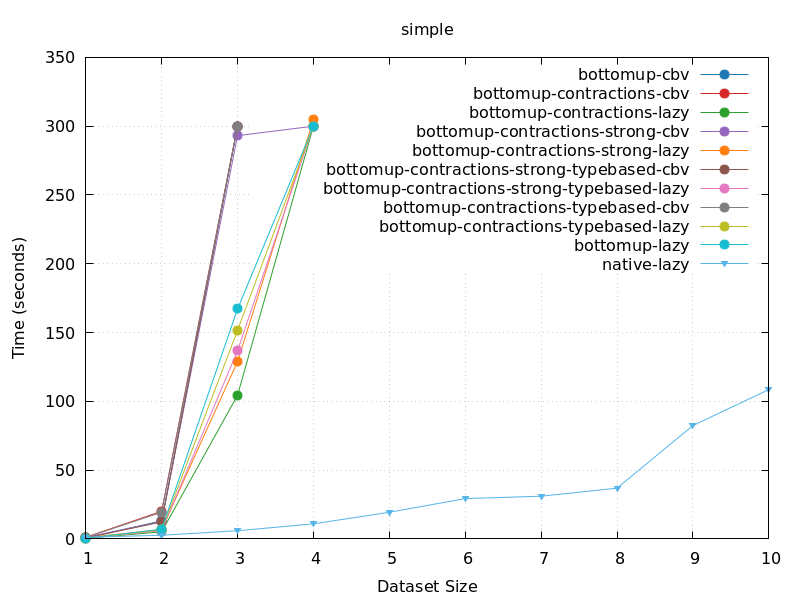
\includegraphics[width=\linewidth]{bottomup.png} 
    \caption{Семейство стратегий \texttt{bottomup}}
    \end{subfigure}
    \begin{subfigure}{0.5\textwidth}
    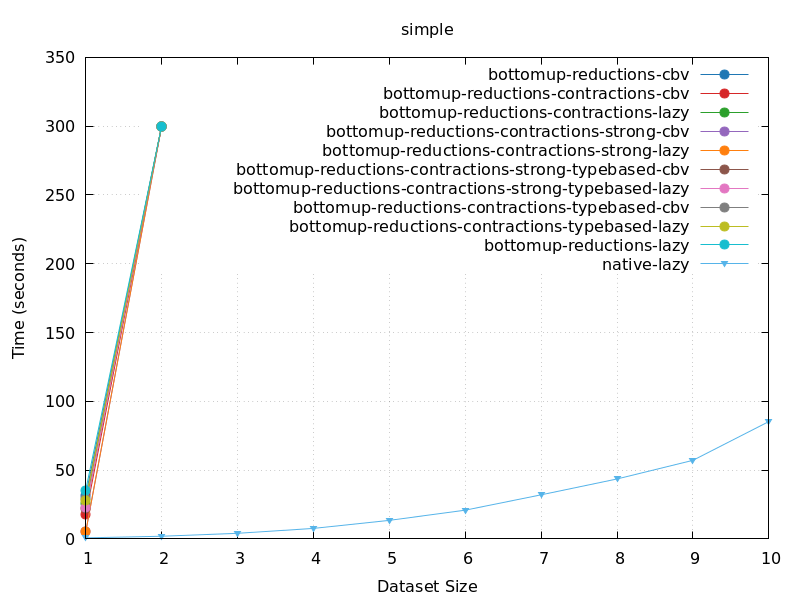
\includegraphics[width=\linewidth]{bottomup_reductions.png}
    \caption{Семейство стратегий \texttt{bottomup-reductions}}
    \end{subfigure}
    \caption{Результаты сравнения стратегий \texttt{bottomup} на наборе данных Simple}
    \label{plot_bottomup}
\end{figure}

Такой резкий рост времени работы для этих стратегий, вероятно, является экспоненциальным, что несложно объяснить. Действительно, стратегия \texttt{bottomup} подставляет все термы не редуцируя их, что приводит к значительной дубликации кода, и даже мемоизация в ленивом вычислении не решает проблему, поскольку ещё до запуска внутренней редукции процедура подстановки термов с дублицированным кодом становится экспоненциальной. То, что стратегия \texttt{bottomup-reductions}, включающей в себя редукции на каждом шаге, является ещё медленнее наивной версии, может показаться контринтуитивным. Однако, этот факт объясняется тем, что при преждевременной редукции термов в стратегии \texttt{bottomup-reductions}, то есть при редукции термов, которые содержат неподставленные свободные переменные $y_i$, терм может значительно увеличиваться в размерах из-за "мёртвого кода", например если такая переменная стоит в голове условного оператора или сопоставления с образцом. 

В более общем смысле, рисунок \ref{plot_bottomup} иллюстрирует, насколько важно выбрать правильный порядок вычислений и подстановок, так как в результате выбора неверного порядка легко получить стратегию, не применимую на практике из-за крайней неэффективности.


\begin{figure}[h]
    \begin{subfigure}{0.5\textwidth}
    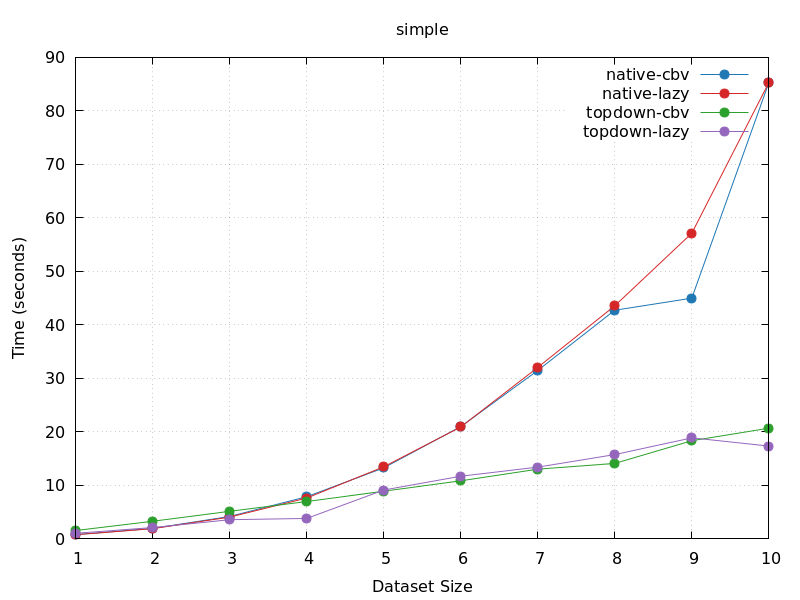
\includegraphics[width=\linewidth]{basic_simple.png} 
    \caption{Набор данных Simple}
    \end{subfigure}
    \begin{subfigure}{0.5\textwidth}
    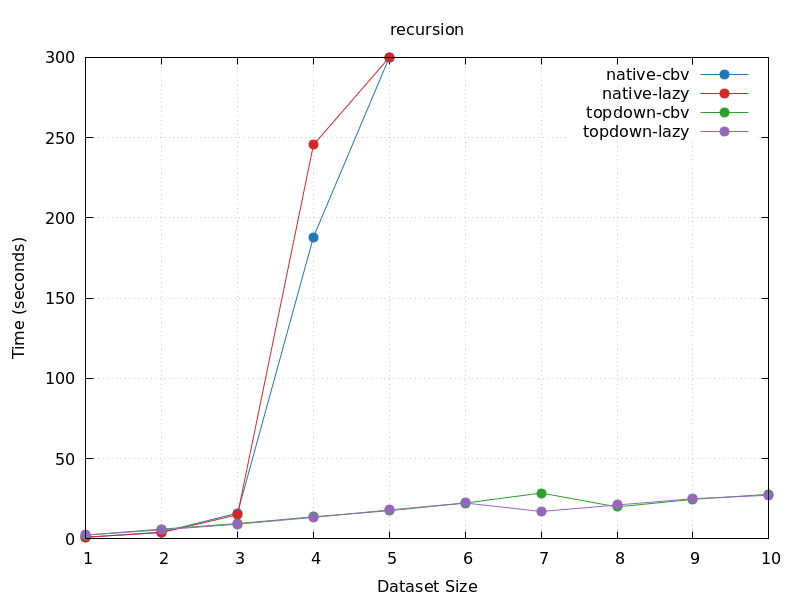
\includegraphics[width=\linewidth]{basic_recursion.png}
    \caption{Набор данных Recursion}
    \end{subfigure}
    \caption{Результаты сравнения базовых стратегий}
    \label{plot_basic}
\end{figure}

Перейдём к сравнению двух оставшихся базовых стратегий, \texttt{native} и \texttt{topdown}. Результаты сравнения этих стратегий на наборах данных Simple и Recursion приведены на рисунке \ref{plot_basic}. Оказывается, что уже базовая стратегия \texttt{topdown} показывает результаты, значительно лучше, чем \texttt{native}. На наборе данных Recursion стратегия \texttt{native} показывает экспоненциальный взрыв, похожий на наблюдаемый со стратегиями \texttt{bottomup}, и вероятно объясняемый неэффективностями в реализации редукций. Однако, стратегия \texttt{topdown} даже без дальнейших эвристических оптимизаций, использующая множество редукций для решения небольших подзадач, не демонстрирует экспоненциального поведения, и даже выглядит линейно на рассматриваемых объёмах данных. Таким образом, уже правильный выбор базовой стратегии, использующую естественную декомпозицию данных на уравнения и обрабатывающих их в необходимом порядке, позволяет значительно улучшить производительность вычислений.

Другим наблюдением, отражённым на рисунке \ref{plot_basic}, является статистическая неразличимость на рассматриваемых программах при использовании внутренних редукций \texttt{cbv} или \texttt{lazy}. Из-за этой неразличимости в приведённых далее графиках и рассуждениях вариации стратегий, отличающиеся только выбором внутренней редукции, будут опущены, и для всех стратегий будет использоваться вариант с редукцией \texttt{lazy}. Однако, было установлено, что на некоторых программах выбор редукции всё же имеет существенное влияние, это будет описано в разделе \ref{lazy_best}.

Итак, стратегия \texttt{topdown} уже показывает значительное, асимптотическое улучшение относительно стратегии \texttt{native}, что является центральным практическим результатом работы. Однако, можно получить ещё более эффективные стратегии, рассмотрев дальнейшие эвристики, описанные в разделах \ref{graphbased} и \ref{typebased}. Результаты сравнения этих стратегий приведены на рисунке \ref{plot_heuristics}.

\begin{figure}[h]
    \begin{subfigure}{0.5\textwidth}
    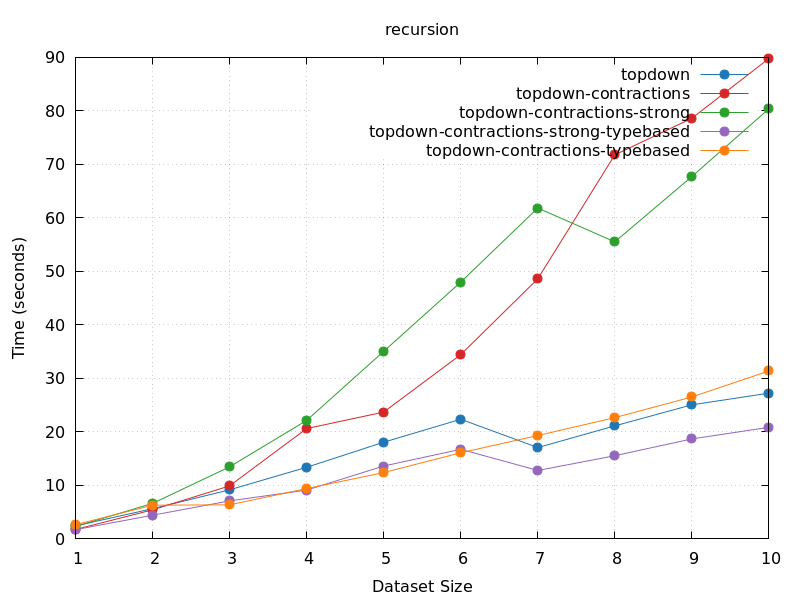
\includegraphics[width=\linewidth]{topdown.png} 
    \caption{Семейство стратегий \texttt{topdown}}
    \label{plot_heuristics_topdown}
    \end{subfigure}
    \begin{subfigure}{0.5\textwidth}
    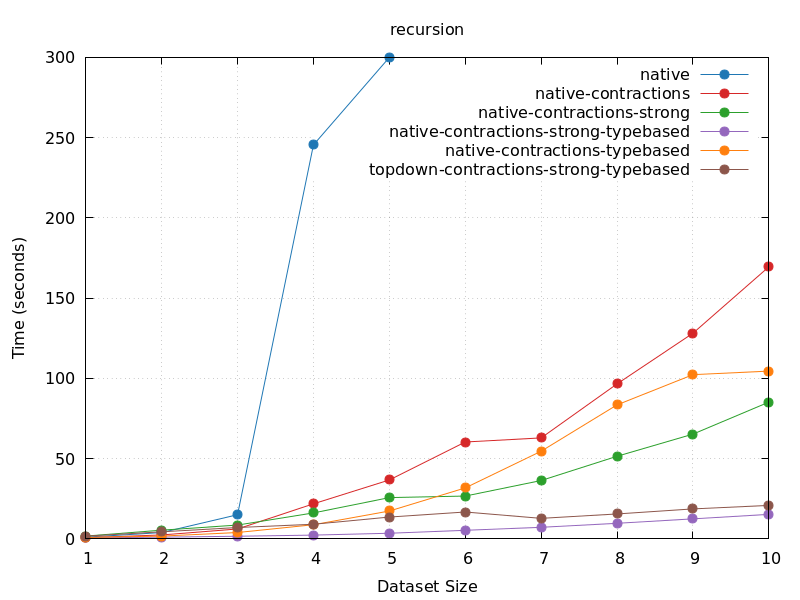
\includegraphics[width=\linewidth]{native.png}
    \caption{Семейство стратегий \texttt{native}}
    \label{plot_heuristics_native}
    \end{subfigure}
    \caption{Результаты сравнения стратегий с эвристическими оптимизациями на наборе данных Recursion}
    \label{plot_heuristics}
\end{figure}

Рассматривая результаты различных эвристических оптимизаций стратегии \\\texttt{topdown} (рис. \ref{plot_heuristics_topdown}), можно заметить, что почти все из них оказывают негативное влияние на производительность. Так, хуже всего результат показывают оптимизации, основанные на чистых графовых свойствах (\texttt{topdown-contractions} и \\\texttt{topdown-contractions-strong}), из-за накладных расходов на явное построение графа они проигрывают базовой стратегии. Не показывает значительного улучшения и слабая версия оптимизации, основанной на типах данных \texttt{topdown-contractions-} \texttt{typebased}. Однако сильная версия этой оптимизации \texttt{topdown-contractions-strong-} \texttt{typebased} немного быстрее, чем базовая версия \texttt{topdown}.

Что же касается тех же оптимизаций, применённых для стратегии \texttt{native} (рис. \ref{plot_heuristics_native}), то они все улучшают эффективность базовой стратегии и не показывают такого резкого роста. Однако, их относительный порядок совпадает с изложенным для \texttt{topdown}, а именно графовые эвристики и слабая версия типовой эвристики показывают не такой эффективный результат, как сильная версия типовой эвристики \texttt{native-contractions-strong-typebased}. Интересно, что несмотря на то, что базовая версия \texttt{native} значительно медленнее базовой версии \texttt{topdown}, если применить к обеим стратегиям оптимизацию \texttt{contractions-strong-typebased}, то \texttt{native} станет даже немного, но статистически заметно, эффективнее \texttt{topdown}.

Итак, выявлены три стратегии, показывающие наилучшие результаты: стратегия \texttt{topdown} в базовой версии и стратегии \texttt{topdown} и \texttt{native} с оптимизацией \texttt{contractions-} \texttt{strong-typebased}. На рисунке \ref{plot_winners} приведены результаты этих трёх стратегий на больших объёмах данных (до n = 40, тогда как предыдущие графики включали данные до n = 10). 

\begin{figure}[h]
    \begin{subfigure}{0.5\textwidth}
    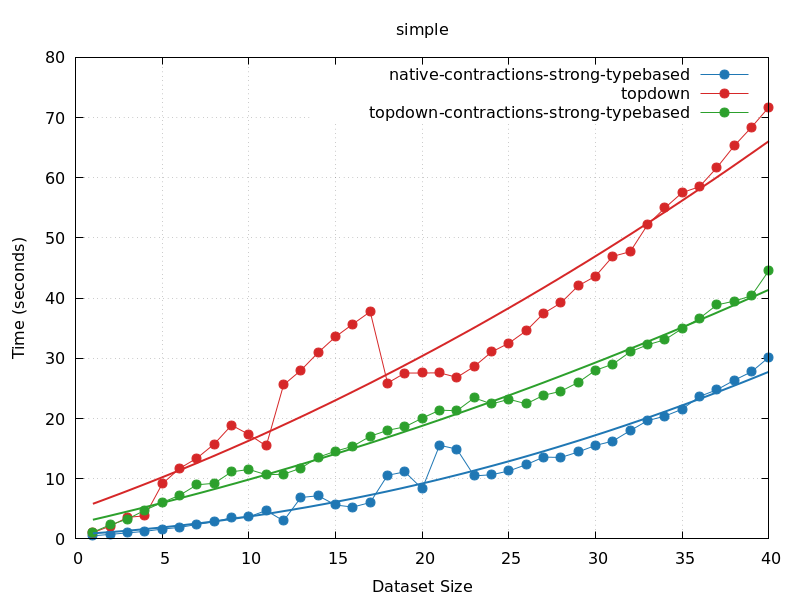
\includegraphics[width=\linewidth]{winners_simple.png} 
    \caption{Набор данных Simple}
    \label{plot_winners_simple}
    \end{subfigure}
    \begin{subfigure}{0.5\textwidth}
    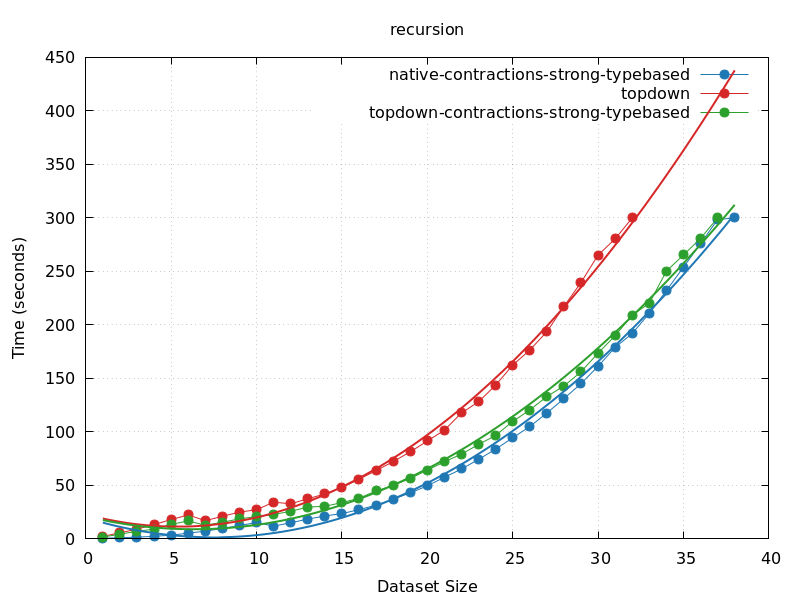
\includegraphics[width=\linewidth]{winners_recursion.png}
    \caption{Набор данных Recursion}
    \label{plot_winners_recursion}
    \end{subfigure}
    \caption{Результаты сравнения лучших стратегий на больших данных}
    \label{plot_winners}
\end{figure}

\begin{figure}[h]
    \begin{subfigure}{0.5\textwidth}
    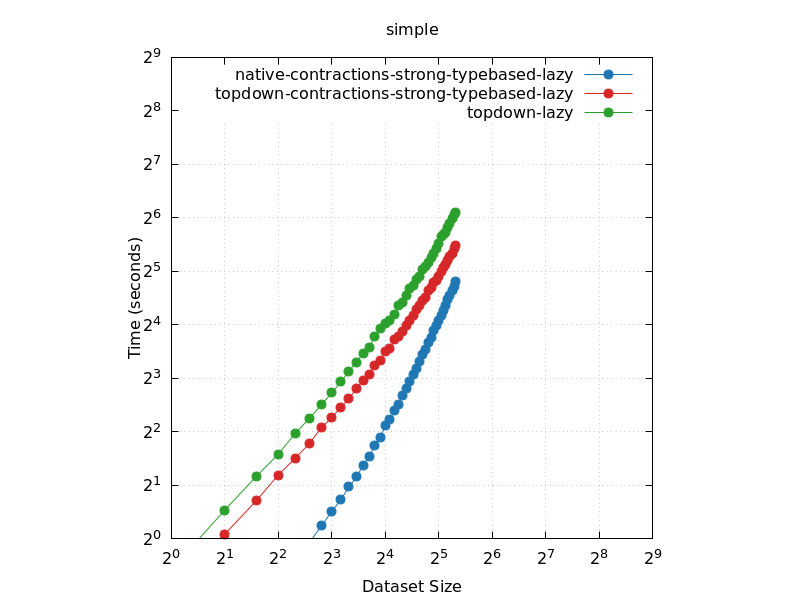
\includegraphics[width=\linewidth]{loglog_simple.png} 
    \caption{Набор данных Simple}
    \label{loglog_simple}
    \end{subfigure}
    \begin{subfigure}{0.5\textwidth}
    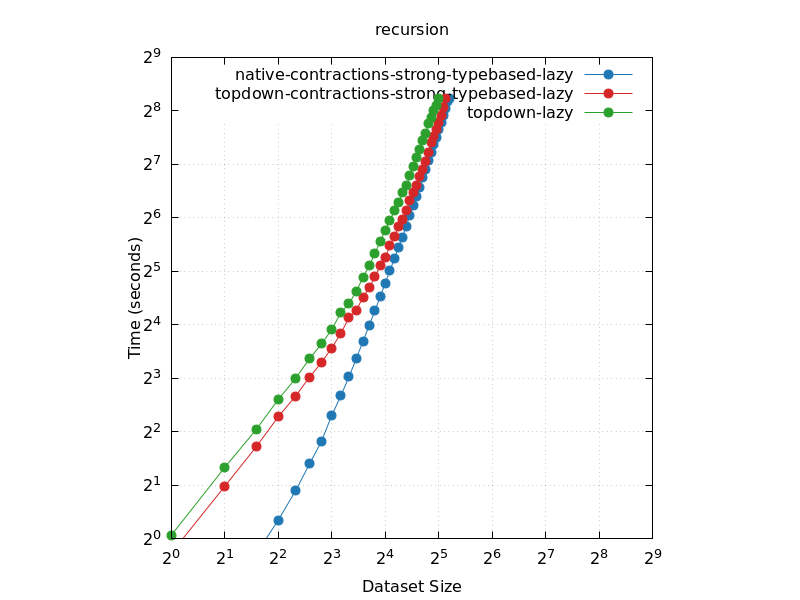
\includegraphics[width=\linewidth]{loglog_recursion.png}
    \caption{Набор данных Recursion}
    \label{loglog_recursion}
    \end{subfigure}
    \caption{Результаты сравнения лучших стратегий на больших данных в log-log шкале}
    \label{plot_loglog}
\end{figure}

На наборе данных Simple (рис. \ref{plot_winners_simple}) рост времени работы стратегий выглядит почти линейным, кривизна графика не очень заметна. Однако, на наборе данных Recursion (рис. \ref{plot_winners_recursion}), который является в несколько раз более вычислительно затратным по размеру системы уравнений, чем набор Simple, отчётливо видно, что рост времени работы всех трёх стратегий имеет нелинейный характер. На рисунке \ref{plot_loglog} приведены версии тех же графиков с рисунка \ref{plot_winners}, но использована log-log шкала. Видно, что рост времени работы всех стратегий является полиномиальным. При этом обе версии стратегии \texttt{topdown} на наборе Simple завершаются за $\mathcal{O}(n^{1.5})$, а на наборе Recursion за $\mathcal{O}(n^2)$. Стратегия \texttt{native-contractions-strong-typebased} на наборе Simple завершается за $\mathcal{O}(n^2)$, а на наборе Recursion за $\mathcal{O}(n^{2.5})$. Интересно, что стратегия, показывающая на рассматриваемых данных лучшие результаты, имеет менее эффективную асимптотику. Из этого следует, что при достаточно больших размерах данных стратегия \texttt{topdown-contractions-strong-typebased}, имеющая асимптотику лучше, будет показывать самые эффективные результаты. Однако, похоже, что это произойдёт лишь при данных крайне большого размера, представляющим меньший практический интерес.

Несмотря на то, что было бы предпочтительнее получить линейный алгоритм, коэффициенты полиномиальных функций, описывающих время работы лучших стратегий, достаточно малы и приемлемы на практике. Так, за пять минут лучшая стратегия может обработать код из нескольких сотен строк кода с глубиной рекурсии до 35, что соответствует реалиям разработки смарт-контрактов. Отметим, что стратегия \texttt{native} без оптимизаций за пять минут может обработать только код из нескольких десятков строк кода с глубиной рекурсии до 4, то есть существенно меньше, и не может обрабатывать за адекватное время большую часть реальных смарт-контрактов.

На всех рассматриваемых наборах данных эффективнее всего проявляет себя стратегия \texttt{native-contractions-strong-typebased}, хотя её преимущество относительно стратегии \texttt{topdown-contractions-strong-typebased} уменьшается с увеличением размеров теста, а на крайне больших тестах вторая стратегия превзойдёт первую. Что же касается преимущества относительно базовой стратегии \texttt{topdown}, то есть преимущества стратегии с эвристическими оптимизациями перед лучшей базовой стратегией, оно может показаться незначительным на больших тестах, поскольку асимптотического выигрыша эвристические оптимизации не привносят и на больших тестах разница между ними не кажется существенной. Однако, на вполне реалистичных размерах функции в 70 строк (n = 35 в наборе данных Simple) и глубине рекурсии в 10, эвристические оптимизации позволяют ускорить вычисление в 3 раза. Такие оптимизации могут быть особенно значимы в случаях, когда символьное вычисление используется в композитных процессах, например при доказательстве свойств сложных сценариев, где этот множитель 3 будет возведён в степень. Таким образом, несмотря на то, что уже базовая стратегия \texttt{topdown} показывает хороший результат, результат дальнейших оптимизаций также значим на практике.

\subsection{Эксперименты на коде с условными операторами}\label{if_experiments}

Перейдём к экспериментам с использованием программ, содержащих условные операторы. Поскольку, как описано в разделе \ref{ifs}, работа с условными операторами в общем случае является экспоненциально сложной относительно числа условных операторов, все графики в этом разделе будут построены на логарифмической шкале. Также из рассмотрения в этом разделе будут исключены стратегии из семейства \texttt{bottomup}, показывающие экспоненциальный рост уже на линейном коде.

\begin{figure}[h]
    \begin{subfigure}{0.5\textwidth}
    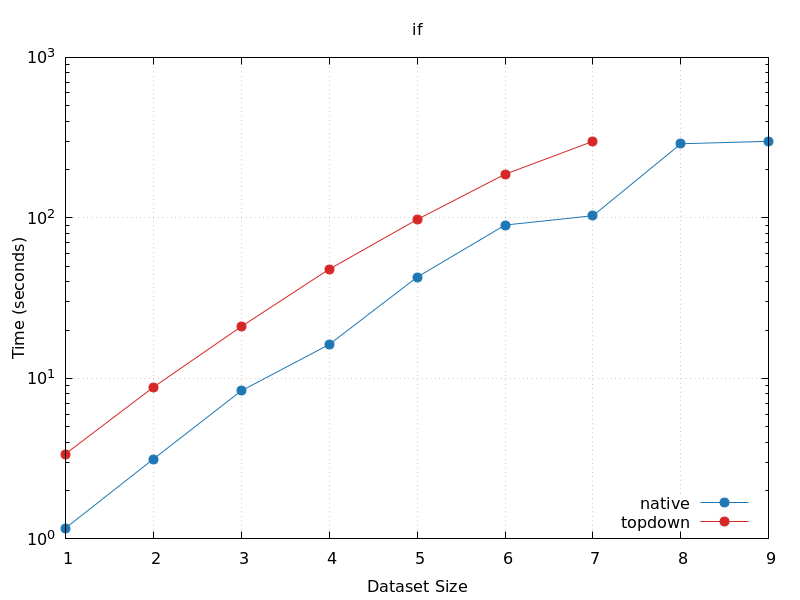
\includegraphics[width=\linewidth]{basic_if.png} 
    \caption{Набор данных If}
    \end{subfigure}
    \begin{subfigure}{0.5\textwidth}
    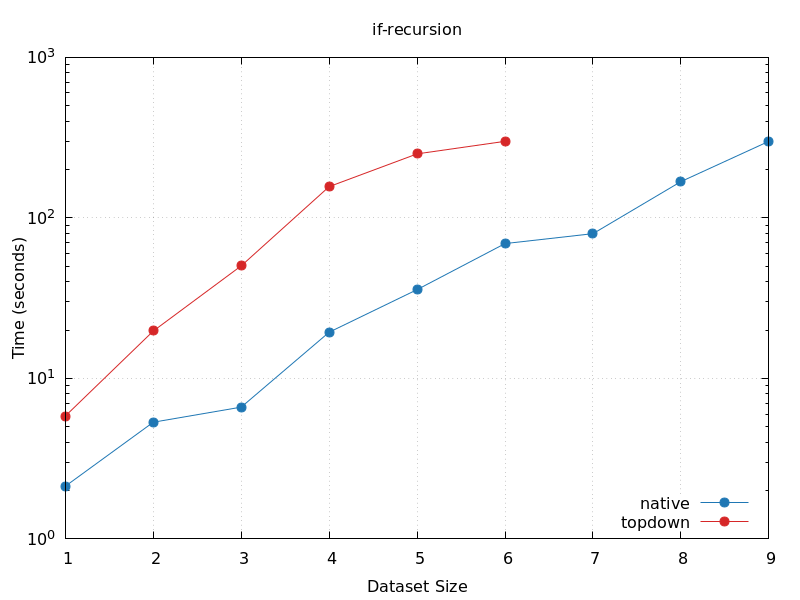
\includegraphics[width=\linewidth]{basic_ifrec.png}
    \caption{Набор данных IfAndRecursion}
    \end{subfigure}
    \caption{Результаты сравнения базовых стратегий на программах с условными операторами}
    \label{basic_ifs}
\end{figure}

На рисунке \ref{basic_ifs} представлены результаты сравнения базовых стратегий \texttt{topdown} и \texttt{native}. Интересно, что на коде, содержащем большое число условных операторов, в отличие от линейных программ, стратегия \texttt{native} показывает более эффективный результат. Это объясняется описанными в разделе \ref{ifs} особенностями работы с условными операторами. Так, при использовании стратегии \texttt{topdown} для сохранения инварианта необходимо вызывать \texttt{destruct}, как только в порядке обработки встречается уравнение с условным оператором, что вызывает экспоненциальное дублирование подстановок в дальнейших уравнениях. 

\begin{figure}[h]
    \begin{subfigure}{0.5\textwidth}
    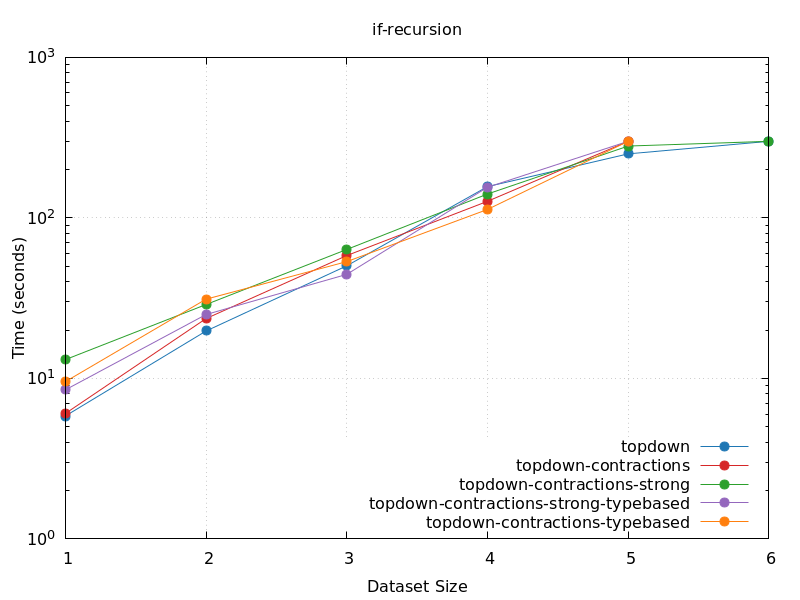
\includegraphics[width=\linewidth]{topdown_ifrec.png} 
    \caption{Семейство стратегий \texttt{topdown}}
    \label{heuristics_ifs_topdown}
    \end{subfigure}
    \begin{subfigure}{0.5\textwidth}
    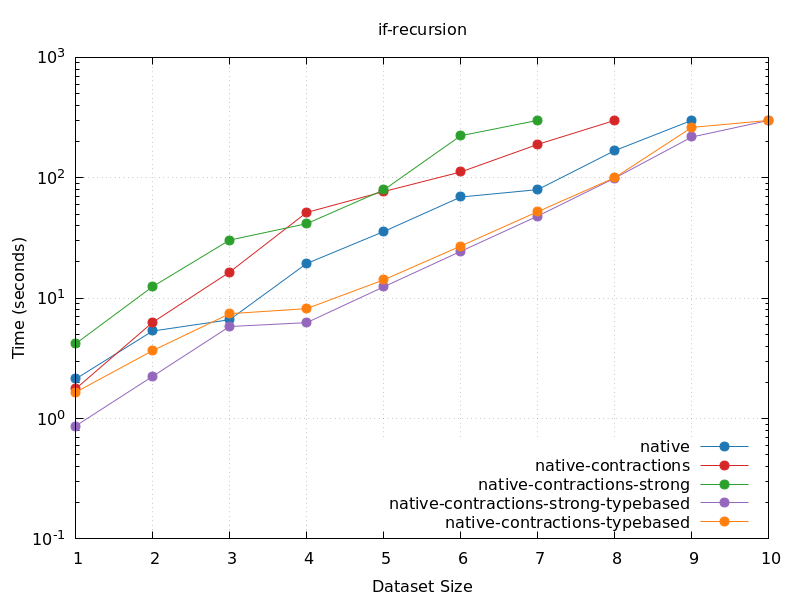
\includegraphics[width=\linewidth]{native_ifrec.png}
    \caption{Семейство стратегий \texttt{native}}
    \label{heuristics_ifs_native}
    \end{subfigure}
    \caption{Результаты сравнения стратегий с эвристическими оптимизациями на наборе данных IfAndRecursion}
    \label{heuristics_ifs}
\end{figure}

На рисунке \ref{heuristics_ifs_topdown} видно, что никакие эвристики не оказывают значимого влияния на эффективность стратегии \texttt{topdown}. Похоже, описанная выше неэффективность в экспоненциальной дубликации подстановок нивелирует потенциальный прирост производительности от эвристических оптимизаций. В то же время, для эвристик, применённых к стратегии \texttt{native} (рисунок \ref{heuristics_ifs_native}), наблюдаются те же закономерности, описанные в предыдущем разделе: эвристики, основанные на графовых свойствах, не демонстрируют улучшения или замедляют работу, а эвристики, основанные на типах данных, улучшают производительность.

В результате можно установить, что, несмотря на то что на программах с условными операторами некоторые менее эффективные на линейном коде стратегии могут оказаться более эффективными из-за особенностей работы с условными операторами, тем не менее самой эффективной стратегией остаётся \texttt{native-contractions-strong-} \texttt{typebased}.

\subsection{Выбор внутренней редукции}\label{lazy_best}

\begin{wrapfigure}{l}{0.5\textwidth}
    \centering
    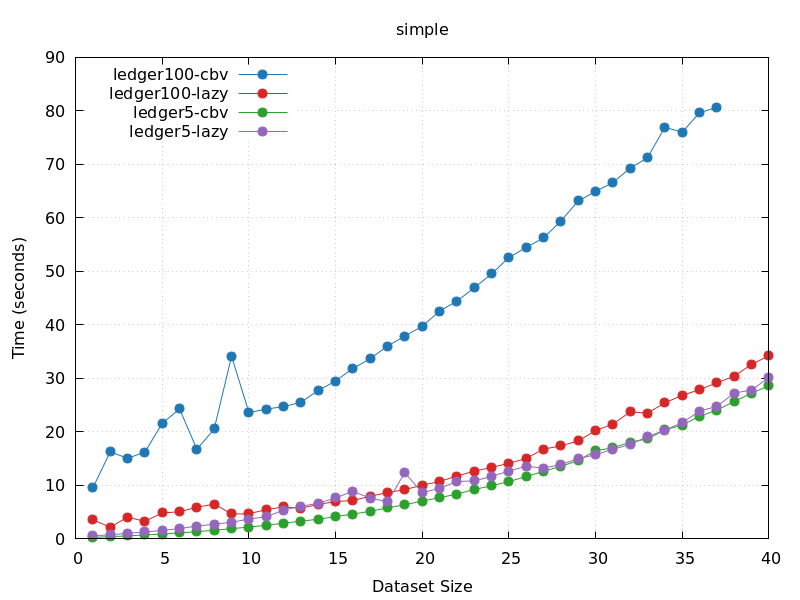
\includegraphics[width=0.5\textwidth]{ledger_size.png} 
    \caption{Результаты сравнения внутренних редукций на разном количестве полей}
    \label{ledger_size}
\end{wrapfigure}

В приведённых ранее графиках и рассуждениях варианты стратегий с внутренней редукцией \texttt{cbv} опускались, так как они не показывали на рассматриваемых программах значительного отличия от вариантов с \texttt{lazy}. Однако, оказалось, что для некоторых программ \texttt{lazy} показывает значительно более эффективный результат.

Напомним, что применение \texttt{lazy} особенно эффективно при редукциях термов, содержащих большое количество "мёртвого кода". Поэтому был проведён эксперимент по запуску лучшей стратегии \texttt{contractions-strong-typebased} на двух версиях набора данных Simple. В первом состояние контракта включало только 5 используемых полей, во втором после добавления 95 неиспользуемых полей общее число полей равняется 100. 

На рисунке \ref{ledger_size} представлены результаты такого эксперимента. Видно, что при малом числе полей, как и наблюдалось в предыдущих экспериментах, выбор внутренней редукции не оказывает значимого влияния на эффективность вычисления. Однако, при увеличении числа полей от 5 до 100 стратегия, основанная на редукции \texttt{cbv}, замедляется в несколько раз (около трёх), тогда как при выборе редукции \texttt{lazy} замедление хоть и заметно, но не является настолько существенным. 

Таким образом, при наличии в вычислении "мёртвого кода" существенного размера в виде неиспользуемых в рассматриваемой функции полей программы, выбор редукции \texttt{lazy} позволяет в несколько раз ускорить алгоритм. Поскольку в рамках исследования не было найдено случаев, в которых редукция \texttt{cbv} показывает заметное ускорение, можно сделать вывод о том, что редукция \texttt{lazy} лучше подходит для рассматриваемой задачи. 

\subsection{Эксперименты на реальных данных}

В синтетических данных, эксперименты на которых описаны выше, изучалось влияние ключевых параметров на эффективность стратегий, будь то размер кода, глубина рекурсии или число условных операторов. В этом разделе будут рассмотрены результаты сравнения стратегий на коде реального смарт-контракта кошелька с мультиподписью.

Для этого был взята спецификация и доказательства трёх ключевых функций этого контракта, \texttt{sendTransaction}, \texttt{submitTransaction} и \texttt{confirmTransaction}. Ключевые характеристики этих функций приводятся в таблице \ref{multisig_analysis}.

\begin{table}[h]
\centering
\begin{tabular}{|c|c|c|c|c|}
\hline
Функция & Строк & Вызовов функций & Глубина рекурсии & Условных операторов \\
\hline
send & 4 & 2 & 1 & 2 \\
\hline
submit & 45 & 15 & 2 & 7\\
\hline
confirm & 22 & 7 & 2 & 4 \\
\hline
\end{tabular}
\caption{Ключевые характеристики рассматриваемых функций}
\label{multisig_analysis}
\end{table}

Внутри доказательства спецификации каждой из функций несколько раз вызывается процедура упрощения системы уравнений с помощью одной из стратегий редукции, для каждого из доказываемых аспектов поведения функций или различных предположений на аргументы функции и исходное состояние системы. Затем, после того как все эти подцели доказаны, вызывается команда QED, производящая финальную проверку типов построенного доказательства.

В таблице \ref{results_multisig} приведены результаты таких экспериментов. Все используемые стратегии включают в себя \texttt{lazy} как внутреннюю тактику, согласно соображениям, высказанным в разделе \ref{lazy_best}. Для экспериментов на этом этапе по результатам экспериментов на синтетических данных были отобраны четыре стратегии: \texttt{native} (NL), \texttt{native-contractions-strong-typebased} (NCSTL), \texttt{topdown} (TL) и \texttt{topdown-}\\\texttt{contractions-strong-typebased} (TCSTL).

\begin{table}[h]
\centering
\subfloat[Функция sendTransaction]{\begin{tabular}{|c|c|c|c|c|}
\hline
\textbf{} & \textbf{NL} & \textbf{NCSTL} & \textbf{TL} & \textbf{TCSTL} \\
\hline
1 & 3.42 & 2.87 & \textbf{2.30} & 5.69 \\
\hline
QED & 2.5 & \textbf{2.39} & 3.8 & 4.53 \\
\hline
$\Sigma$ & 5.92	& \textbf{5.26} & 6.1 & 10.22 \\
\hline
\end{tabular}}
\quad
\subfloat[Функция submitTransaction]{\begin{tabular}{|c|c|c|c|c|}
\hline
\textbf{} & \textbf{NL} & \textbf{NCSTL} & \textbf{TL} & \textbf{TCSTL} \\
\hline
1 & 0.90 & \textbf{0.90} & 1.46 & 1.24 \\
\hline
2 & 0.95 & \textbf{0.84} & 1.05 & 1.04 \\
\hline
3 & 0.99 & \textbf{0.94} & 1.44 & 1.43 \\
\hline
4 & 1.86 & \textbf{1.51} & 3.58 & 2.93 \\
\hline
5 & 1.44 & \textbf{1.22} & 12.26 & 7.99 \\
\hline
6 & 23.40 & \textbf{7.46} & 46.16 & 58.54 \\
\hline
7 & 23.63 & \textbf{7.75} & 41.19 & 58.16 \\
\hline
QED & \textbf{11.51} & 12.63 & 78.09 & 87.26 \\
\hline
$\Sigma$ & 64.68 & \textbf{33.25} & 185.23 & 218.59 \\
\hline
\end{tabular}}
\quad
\subfloat[Функция confirmTransaction]{\begin{tabular}{|c|c|c|c|c|}
\hline
\textbf{} & \textbf{NL} & \textbf{NCSTL} & \textbf{TL} & \textbf{TCSTL} \\
\hline
1 & 0.69 & 0.65 & \textbf{0.53} & 0.49 \\
\hline
2 & 0.78 & \textbf{0.70} & 1.03 & 0.70 \\
\hline
3 & 0.10 & \textbf{0.09} & 0.11 & 0.10 \\
\hline
4 & 1.73 & \textbf{1.44} & 1.62 & 2.08 \\
\hline
5 & 1.79 & \textbf{1.25} & 3.03 & 2.20 \\
\hline
6 & \textbf{0.20} & 0.22 & \textbf{0.20} & \textbf{0.20} \\
\hline
7 & 2.08 & \textbf{1.35} & 3.47 & 2.53 \\
\hline
8 & 3.64 & \textbf{2.03} & 5.68 & 4.65 \\
\hline
9 & 16.80 & 12.33 & 12.86 & \textbf{11.79} \\
\hline
QED & \textbf{10.25} & 10.34 & 31.74 & 26.73 \\
\hline
$\Sigma$ & 38.06 & \textbf{30.4} & 60.27	& 51.47 \\
\hline
\end{tabular}}
\caption{Результаты экспериментов на реальных данных}
\label{results_multisig}
\end{table}

Стратегии класса \texttt{topdown} показывают неэффективные результаты. Вероятно, это связано с теми же причинами, по которым они работали относительно медленно в экспериментах в разделе \ref{if_experiments}. Во всех рассматриваемых функциях присутствуют условные операторы в достаточном количестве, а с ними эти стратегии работают менее эффективно. Такая неэффективная работа этих стратегий на реальных данных является дополнительным аргументом против их использования на практике, несмотря на то, что, как показано в разделе \ref{main_results}, стратегии из класса \texttt{topdown} на некоторых примерах могут показывать лучшую асимптотику.

Что же касается двух оставшихся стратегий, базовой стратегии \texttt{native} и самой эффективной стратегии \texttt{native-contractions-strong-typebased}, вторая не демонстрирует такого серьёзного улучшения относительно первой, как наблюдалось в некоторых тестах из раздела \ref{main_results}. По-видимому, при таких характеристиках кода, как небольшая глубина рекурсии и большое число условных операторов, эвристики не дают такого серьёзного улучшения. Однако, это улучшение всё ещё значительно: так, на запусках 6 и 7 функции \texttt{submitTransaction} эвристика улучшает результат стратегии \texttt{native} в три раза, а на запуске 9 функции \texttt{confirmTransaction}~--- в полтора.

Более того, не нашлось ни одного запуска, в котором какая-то стратегия была бы заметно эффективнее \texttt{native-contractions-strong-typebased}. Эксперименты из предыдущих разделов также не находили таких случаев (за исключением, возможно, крайне больших и менее интересных на практике размеров кода). Ни про какие другие стратегии этого сказать нельзя. Таким образом, несмотря на то, что для каких-то программ выигрыш от использования этой стратегии может быть менее заметен, нет необходимости выбирать стратегию исходя из свойств рассматриваемой программы, ведь единственная стратегия на всех экспериментах показывает результаты не хуже остальных.

\subsection{Выводы и результаты по главе}

Создан тестовый набор из синтетической части (четыре программы на языке Ursus линейно растущего размера, покрывающие фундаментальные конструкции языков программирования) и реальной части (смарт-контракт из практики компании\\Pruvendo). По результатам экспериментов с запуском стратегий на тестах можно сделать следующие выводы:

\begin{itemize}
    \item все стратегии класса \texttt{bottomup} экспоненциальны и неприменимы на практике; 
    \item базовая стратегия \texttt{topdown} на линейном коде уже значительно эффективнее, чем \texttt{native}; 
    \item графовые эвристики и слабая версия эвристики на типах данных оказывает отрицательное влияние или незначительное положительное влияние на эффективность стратегий;
    \item лучшие результаты на линейном коде показывает стратегия \texttt{native} с применённой эвристикой \texttt{contractions-strong-typebased}, при этом стратегия \texttt{topdown} в базовой версии или с применённой эвристикой имеют лучшую асимптотику, однако будут более эффективными лишь на крайне больших данных;
    \item лучший результат на коде с условными операторами показывает стратегия \texttt{native} с применённой эвристикой \texttt{contractions-strong-typebased}, тогда как все стратегии из класса \texttt{topdown} на таком коде хуже даже базовой стратегии \texttt{native};
    \item стратегия \texttt{native-contractions-strong-typebased-lazy} является особо эффективной в программах с большой глубиной рекурсии и малым числом условных операторов, однако на всех исследуемых программах эта стратегия не показывала результат заметно хуже любой другой стратегии;
    \item итого, лучшей стратегией по всем экспериментам является \\\texttt{native-contractions-strong-typebased-lazy}.
\end{itemize}

\end{document}
